%%% Research Diary - Entry
\documentclass[11pt,a4paper]{article}

% Working date: The date this entry is describing. Not necessary the date of last edit.
\newcommand{\workingDate}{\textsc{2019 $|$ April $|$ 30}}

% Name and institution must preceed call to researchdiary.sty package
\newcommand{\userName}{Pierre Bréchet}
\newcommand{\institution}{TUM}

% The guts and glory
\usepackage{research_diary}
\usepackage{usrcmd}
\bibliography{bibliography}

% Begin document.
% Use \logoPNG or \logoEPS. If compiling with PDFTeX, use \logoPNG
\begin{document}
% \logoPNG

{\Huge April 30}

\section*{Sinkhorn loss}

For $X=Y$, $\alpha \in \Mpo(X), \beta \in \Mpo(X)$, the Wasserstein loss based on the $\Wce$ is defined as:
\begin{align}
    \label{eqn:wasserstein-loss}
    \Wce(\alpha, \beta) &= \min_{\gamma} \set{ \int_{\XX} c(x, y) \d \gamma(x, y) + \eps \R(\gamma) \st \gamma \in \Pi(\alpha, \beta)} \\
                        &= \min_{\gamma} \int_{\XX} c(x, y) \d \gamma(x, y) + \eps \R(\gamma) + \delta_{\set{\alpha}}\paren{ \pf{\proj{1}}\gamma } + \delta_{\set{\beta}}\paren{\pf{\proj{2}}\gamma} + \delta_{+}(\gamma)
\end{align}

Then, the Sinkhorn loss is defined as:
\begin{equation}
    \SLce(\alpha, \beta) = 2\cdot \Wce(\alpha, \beta) - \Wce(\alpha, \alpha) - \Wce(\beta, \beta)
\end{equation}

The Sinkhorn ROTGAN is defined on the Sinkhorn primal loss
\begin{align}
    &\min_{G} \SLce(\pf{G}{\zeta}, \nu)  \\
    \iff & \min_{G} 2 \cdot \Wce(\pf{G}{\zeta}, \nu) - \Wce(\pf{G}{\zeta}, \pf{G}{\zeta}) - \Wce(\nu, \nu)
\end{align}
%
% \begin{rem}
%     When performing the change of variable $\gammab = \pf{(G, \id)}\gamma$ in $\Wce(\mu, \nu)$
%     \begin{align}
%         &\min_{G}{\Lc(\pf{G}{\mu}, \nu)} &\\
%         %\min_{G}{\int_{\ZX}{c(G(z), y)\d \gamma} &\\
%             \iff &\min_{G} \min_{\gammab} \set{\int_{\XX}{c(x, y) \d \gammab(x, y)} \st \gammab \in \Gamma(\mu, \nu)} & \\
%             \iff & \begin{array}{*2{>{\displaystyle}l}}
%                 \min_{G} \min_{\gammab} &\int_{\XX}{c(x, y) \d \gammab(x, y)}+ \delta_{+}(\gammab) \\
%                                         &+ \delta_{\set{\mu}}(\pf{( \proj{1} )}{ \gammab })  + \delta_{\set{\nu}}(\pf{(\proj{2})}{\gammab})
%             \end{array} \\
%                 \iff & \begin{array}{*2{>{\displaystyle}l}}
%                     \min_{G} \min_{\gamma} &\int_{\XX}{c(x, y) \d \paren{\pf{\paren{G, \id}}{\gamma}}(z, x)}  + \delta_{+}\paren{ \pf{\paren{G, \id}}{\gamma} }\\
%                                            &+ \delta_{\set{\mu}}\paren{ \pf{( \proj{1} )}{\pf{\paren{G,\id}}{\gamma}} }  + \delta_{\set{\nu}}\paren{ \pf{(\proj{2})}{\pf{\paren{G, \id}}{\gamma}} }
%                 \end{array} &\gammab = \pf{(G, \id)}{\gamma}\label{eqn:otgan-cv} \\
%         % \min_{\gammab} \int_{\XX}{c(x, y) \d \gammab(x, y)} + \eps R(\gammab)
%             \iff &\begin{array}{*2{>{\displaystyle}l}}
%                 \min_{G} \min_{\gamma} &\int_{\XX}{c(G(z), y) \d \gamma}(z, y) + \delta_{+}\paren{\gamma } \\
%             % &+ \delta\set{\pf{(\proj{1}}{\pf{(G, \id)}{\gamma}} = \pf{G}{\zeta}, \pf{\projY}{\pf{(G, \id)}{\gamma}} = \nu)}
%               &+ \delta_{\set{\pf{G}{\zeta}}}\paren{ \pf{( \proj{1}
%               )}{\pf{\paren{G,\id}}{\gamma}} }  + \delta_{\set{\nu}}\paren{ \pf{(\proj{2})}{\pf{\paren{G, \id}}{\gamma}} }
%         \end{array}
%     \end{align}
% \end{rem}
% \section*{Change of variable}
%
% \begin{fac}
%     Let $\alpha, \beta \in \Mpo(X)$ be two measures and let $T: X \to Y$ be a surjective operator such that $\pf{T}\alpha \ll \pf{T}\beta$. Then, $\alpha \ll \beta$ and
%     \begin{equation}
%         \forall x \in X, \quad \radon{\alpha}{\beta}(x) = \radon{\pf{T}{\alpha}}{\pf{T}\beta} \circ T(x)
%     \end{equation}
% \end{fac}
%
% \begin{proof}
%     It follows from the definitions of the push-forward measure and the Radon-Nikodym derivative. Let $h \in \C(Y)$ be any continuous function. The quantity $\int_{Y}h(y) \d \pf{T}{\alpha}(y)$ is computed in two different ways.
%     \begin{align}
%         \forall h \in C(Y),\quad \int_{Y}h(y) \d \pf{T}{\alpha}(y) &= \int_{X}h \circ T(x)\d \alpha(x)\\ %= \int_{X} h \circ T(x) \radon{\alpha}{\beta}(x) \d \beta(x) \\
%         \forall h \in C(Y), \quad \int_{Y}h(y) \d \pf{T}{\alpha}(y) &= \int_{Y}h(y)
%         \radon{\pf{T}{\alpha}}{\pf{T}{\beta}}(y) \d \pf{T}{\beta} = \int_{X}h \circ T (x) \radon{\pf{T}{\alpha}}{\pf{T}{\beta}} \circ T(x) \d \beta(x)
% \end{align}
% Hence
% \begin{equation}
%     \forall h \in \C(Y),\quad \int_{X} h \circ T(x) \d \alpha(x) = \int_{X}h \circ T (x) \radon{\pf{T}{\alpha}}{\pf{T}{\beta}} \circ T(x) \d \beta(x)
% \end{equation}
% Now, since $\forall T: X \to Y,\, \text{T surjective},\, \forall g \in \C(X),\, \exists h \in \C(Y) \st \quad h \circ T = g$ (take $h: y=T(x_0) \mapsto g(x_0)$, $h$ is continuous since $h^{-1}(U) = g^{-1}(U)$ is open for open $U$ since $g$ is contiuous, $x_0$ exists for all $y \in Y$ since $T$ is surjective), we have
%
% \begin{equation}
%     \forall g \in \C(X), \quad \int_{X} g(x) \d \alpha(x) = \int_{X}g(x) \radon{\pf{T}{\alpha}}{\pf{T}{\beta}} \circ T(x) \d \beta(x)
% \end{equation}
% Then, $\alpha \ll \beta$ and by
% definition of the Radon-Nikodym derivative $\radon{\alpha}{\beta} = \radon{\pf{T}{\alpha}}{\pf{T}{\beta}}\circ T$
% \end{proof}
%
% If $\gammab$ solves the OT problem betwenn $\mu = \pf{G}{\zeta}$ and $\nu$ the
% empirical distribution, performng the change of variable $\gamma =
% \pf{(G,\id)}\gammab \eqdef \pf{T}{\gammab}$ results in a change in the
% transport plan densitiy
% \begin{equation}
%     \radon{\gamma}{\zetaxnu} = \radon{\pf{(G, \id)}\gamma}{\pf{( G, \id )}{(\zetaxnu)}}\circ (G, \id) = \radon{\gammab}{\muxnu} \circ (G, \id)
% \end{equation}

% \begin{align}

% Using the extraction feature would correspond to solving
% \begin{align}
%     &\max_{F} \min_{G} \SL(\pf{F}{\pf{G}{\zeta}}, \pf{F}{\nu}) \\
%     \iff & \max_{F} \min_{G} 2 \Wce(\pf{F}{\pf{G}{\zeta}}, \pf{F}{\nu}) - \Wce(\pf{F}{\pf{G}{\zeta}}, \pf{F}{\pf{G}{\zeta}}) - \Wce(\pf{F}{\nu}, \pf{F}{\nu})
% \end{align}

\section{Informative Regularization}
The informative variant primal reads
\begin{align}
    % \tag{Ent-ROTGAN}
     \label{eqn:info-rotgan}
     % \tag{IROTGAN}
     &\begin{array}{*2{>{\displaystyle}l}}
         \min_{G} \min_{\gamma}  &\int_{\ZY}{ c(G(z), y) \d \gamma(z, y)}  + \eps \R(\gamma)
    - \lambda_1 \KL{\pf{(\projZAX)}{\gamma}}{\oprod{\zeta_1}{\nu}}\\
                                 &+ \delta_{\set{\pf{G}{\zeta}}}\paren{\pf{( \proj{1} )}{\pf{(G, \id)}{\gamma}}} + \delta_{\set{\nu}}\paren{\pf{( \proj{2} )}{\pf{(G, \id)}{\gamma}}}
     \end{array} \\
     \iff &\min_{G} \Wice(\pf{G}\zeta, \nu)
\end{align}

\begin{rem}
    Since $\Wice(\pf{G}\zeta, \pf{G}\zeta)$ and $\Wice(\nu, \nu)$ are not
    defined, we would like to express the informative variant of the Sinkhorn
    Loss without (defining them would require additional neural networks
    (2 more?))
\end{rem}

For $F(\eta) \eqdef \lambda_1 \KL{\eta}{\oprod{\zeta_1}{\nu}}$ we have
$-\conj{\paren{\conj{F}}}(\eta) = -F(\eta) = \min_{Q_1}{-\int_{\ZBX} {Q_1(z_1, y)
\d \eta} + \lambda_1 F^{\star}( Q_1 / \lambda_1 )}$, hence the new network $Q_1$.

Allowing $\min = \inf$ and swapping $\min_{Q_1}$ with $\min_{\gamma}$,

\begin{align}
    &\begin{array}{*2{>{\displaystyle}l}}
        \min_{G} \min_{\gamma} \min_{Q_1} &\int_{\ZY}{c(G(z), y) \d \gamma(z, y)}  + \eps \R(\gamma) + \delta_{\set{\pf{G}{\zeta}}}\paren{\pf{( \proj{1} )}{\pf{(G, \id)}{\gamma}}} + \delta_{\set{\nu}}\paren{\pf{( \proj{2} )}{\pf{(G, \id)}{\gamma}}}
\\
     & - \int_{\ZAX}{Q_1(z_1, y) \d \pf{( \projZAX )}{\gamma}} + \lambda_1 \int_{\ZAX}{\exp{\frac{Q_1(z_1, y)}{\lambda_1}} \d \oprod{\zeta_1 }{\nu (z_1, y)}}
\end{array} \\
    \iff &\begin{array}{*2{>{\displaystyle}l}}
        \min_{G, Q_1} \min_{\gamma} &\Big\{\int_{\ZY}{\bkt{c(G(z), y) - Q_1(z_1, y)}\d \gamma(z, y)}  + \eps \R(\gamma) \\
                                    &+ \delta_{\set{\pf{G}{\zeta}}}\paren{\pf{( \proj{1} )}{\pf{(G, \id)}{\gamma}}} + \delta_{\set{\nu}}\paren{\pf{( \projY )}{\pf{(G, \id)}{\gamma}}}\Big\} \\
     & + \lambda_1 \int_{\ZAX}{\exp{\frac{Q_1(z_1, y)}{\lambda_1}} \d \oprod{\zeta_1 }{\nu (z_1, y)}}
         % + \delta\set{\pf{\proj{1}}{\pf{(G, \id)}{\gamma}} = \pf{G}{\zeta}} + \delta\set{\pf{\projY}{\pf{(G, \id)}{\gamma}} = \nu} \\
\end{array} \\
        \iff & \min_{G, Q_1} \W_{c - Q_1}^{\eps}(\pf{G}{\zeta}, \nu)+ \lambda_1 \int_{\ZAX}{\exp{\frac{Q_1(z_1, y)}{\lambda_1}} \d \oprod{\zeta_1 }{\nu (z_1, y)}}\\
        \iff & \min_{G} \Wice(\pf{G}\zeta, \nu)
\end{align}

Optimal transport plan is recovered through
\begin{align}
    \label{eqn:primal-dual-info-rotgan}
    \radon{\gamma}{\zetaxnu}(z,y)
              &= \left\{ \begin{array}{*2{>{\displaystyle}l}}
                      \exp\paren{\frac{D_1 \circ G(z) + D_2(y) - c(G(z), y) + Q_1(z_1, y)}{\eps}} & \text{if $\R = \Rent$}  \\
                      \frac{\posi{D_1 \circ G(z) + D_2(y) - c(G(z), y) + Q_1(z_1, y)}}{2\eps} & \text{if $\R = \Rtwo$}
              \end{array} \right.
\end{align}

The informative variant of Sinkhorn loss-like $\SLice$ is implemented as
\begin{align}
    &\min_{G} \SLice(\pf{G}{\zeta}, \nu) = 2 \cdot \Wice(\pf{G}{\zeta}, \nu) - \Wce(\pf{G}{\zeta}, \pf{G}{\zeta}) \\%- \Wce(\nu, \nu)
\iff &\boxed{\min_{G} 2 \cdot \min_{Q_1}\set{ \W_{c - Q_1}^{\eps}(\pf{G}{\zeta}, \nu)+ \lambda_1 \int_{\ZAX}{\exp{\frac{Q_1(z_1, y)}{\lambda_1}} \d \oprod{\zeta_1 }{\nu (z_1, y)}}} - \Wce(\pf{G}{\zeta}, \pf{G}{\zeta})}
\end{align}

\begin{rems}
    \begin{itemize}
        \item change $\Wce(\pf{G}{\zeta}, \pf{G}\zeta)$ to $\W_{c-Q_1}^{\eps}(\pf{G}{\zeta}, \pf{G}\zeta)$ ? would turn into

\begin{align}
    &\min_{G} \min_{Q_1} 2 \cdot\W_{c - Q_1}^{\eps}(\pf{G}{\zeta}, \nu)- \W_{c-Q_1}^{\eps}(\pf{G}{\zeta}, \pf{G}\zeta) + \lambda_1 \int_{\ZAX}{\exp{\frac{Q_1(z_1, y)}{\lambda_1}} \d \oprod{\zeta_1 }{\nu (z_1, y)}} \\
    \iff & \min_{G}\min_{Q_1} 2 \cdot \SL_{c-Q_1}^{\eps}(\pf{G}{\zeta}, \nu)+ \lambda_1 \int_{\ZAX}{\exp{\frac{Q_1(z_1, y)}{\lambda_1}} \d \oprod{\zeta_1 }{\nu (z_1, y)}}
\end{align}
    \end{itemize}
\end{rems}

\section{Anti-informative Regularization}

The anti-informative primal reads
\begin{align}
    % \tag{Ent-ROTGAN}
     \label{eqn:anti-info-rotgan}
     % \tag{AROTGAN}
&\begin{array}{*2{>{\displaystyle}l}}
         \min_{G} \min_{\gamma}  &\int_{\ZY}{ c(G(z), y) \d \gamma(z, y)}  + \eps \R(\gamma)
    + \lambda_2 \KL{\pf{(\projZBX)}{\gamma}}{\oprod{\zeta_2}{\nu}}\\
                                 &+ \delta_{\set{\pf{G}{\zeta}}}\paren{\pf{( \proj{1} )}{\pf{(G, \id)}{\gamma}}} + \delta_{\set{\nu}}\paren{\pf{( \projY )}{\pf{(G, \id)}{\gamma}}}
     \end{array} \\
     \iff & \min_{G} \Wace(\pf{G}{\zeta}, \nu)
    % \begin{split}
    % \min_{G} \min_{\gamma}  \int_{\ZY}{ c(G(z), y) \d \gamma(z, y)}  + \eps \R(\gamma)
    % + \lambda_2 \KL{\pf{(\projZBX)}{\gamma}}{\oprod{\zeta_2}{\nu}}\\
    %                    + \delta \set{\pf{\proj{1}}{\pf{(G, \id)}{\gamma}} = \pf{G}{\zeta}, \pf{\projY}{\pf{(G, \id)}{\gamma}} = \nu}
    % \end{split}
\end{align}

\subsection{Derivation with double conjugate of KL}

Again, for $
F(\eta) \eqdef
\lambda_2 \KL{\eta}{\oprod{\zeta_2}{\nu}}$ we have
$\conj{\paren{\conj{F}}}(\eta) = F(\eta) = \sup_{Q_2}{\int_{\ZBX} {Q_2(z_2, y) \d \eta} - \lambda_2 F^{\star}( Q_2 / \lambda_2 )}$
and

\begin{equation}
    % \tag{Ent-ROTGAN}
    \label{eqn:anti-info-rotgan-bis}
    % \tag{AROTGAN}
    \begin{array}{*2{>{\displaystyle}l}}
        \min_{G} \min_{\gamma} \max_{Q_2} &\int_{\ZY}{ \bkt{c(G(z), y) + Q_2(z_2, y)}\d \gamma(z, y)}  + \eps \R(\gamma)- \lambda_2 \int_{\ZBX}{\exp{\frac{Q_2(z_2, y)}{\lambda_2}} \d \oprod{\zeta_2}{\nu}(z_2, y)} \\
                                          &+ \delta_{\set{\pf{G}{\zeta}}}\paren{ \pf{\proj{1}}{\pf{(G, \id)}{\gamma}} } + \delta_{\set{\nu}}\paren{\pf{\projY}{\pf{(G, \id)}{\gamma}}}
                  \end{array}
\end{equation}

% With dual
%
% \begin{equation}
%     \label{eqn:dual-anti-info-rotgan}
% \begin{array}{*2{>{\displaystyle}l}}
%     \max_{D_1, D_2, Q_2} & \int_{Z} {D_1 \circ G(z) \d \zeta(z)} + \int_{X}{D_2(y) \d
%         \nu(y)} \\
%                          & - \lambda_2 \int_{\ZBX}{\exp{\frac{Q_2(z_2, y)}{\lambda_2}} \d \oprod{\zeta_2}{\nu}} \\
%         & - \left\{
%     \begin{array}{*2{>{\displaystyle}l}}
%         \eps \int_{\ZY}{\exp{\paren{\frac{D_1 \circ G(z) + D_2(y) - c(G(z), y) - Q_2(z_2,y)}{\eps}}} \d \zetaxnu(z, y)} &\text{if $\R = \Rent$} \\
%         \frac{1}{2\eps} \int_{\ZY}{ \posi{D_1 \circ G (z) + D_2(y) - c(G(z), y) - Q_2(z_2,y)}^2 \d \zetaxnu(z, y)} & \text{if $\R=\Rtwo$}
% \end{array} \right. \\
%         &\eqdef \L_2(D_1, D_2, Q_2, G)
%     \end{array}
% \end{equation}

\begin{rems}
    \begin{itemize}
        \item The $\sup$ has been changed to $\max$ since we perform stochastic updates of parametrized models
        \item This time, the update of the $Q_2$ network is perfomed jointly with
$D_1,\,D_2$, motivated by the derivation using Fenchel-Rockaffelar theorem
directly on the convex  primal. But using this formulation, the update of $Q_2$ does not need to be jointly made with $D_1, D_2$. One idea would indeed be to invert $\min$ and $\max$, and update $Q_2$ as was $Q_1$ separatly.
\end{itemize}
\end{rems}

Link with derivation using hte Fenchel Rockafellar theorem ?

% Therefore, the primal plan $\gamma$ learned differs for $\Wace(\pf{G}{\zeta}, \pf{G}{\zeta})$ and $\SLace(\nu, \nu) \neq 0$

\subsection{Derivation using the Fenchel Rockafellar theorem}

The primal objective is convex, hence the Fenchel Rockafellar theorem can be directly used.
\begin{itemize}
\item With \begin{equation}\G(\gamma) = \int_{\XY} c(x,y) \d \gamma(x,y) + \eps
    \R(\gamma) + \delta_{+}(\gamma)\end{equation}
    $\G$ and its conjugate
    $\conj{\G}$ are the same as when no informative regularization is used (depends on $\R$).

    \item
        With
        \begin{equation}
            \F(\phi, \chi, \psi) = \delta_{\set{\mu}}(\phi) + \delta_{\set{\nu}}(\chi) + \lambda_2 \KL{\psi}{\zeta_2 \otimes \nu}
        \end{equation}
        we have
        \begin{equation}
        \conj{\F}(u, v, w) = \int_{X}u(x) \d \mu(x) + \int_{X} v(y) \d \nu(y) + \lambda_2 \int_{Z_2 \times X} \exp{\frac{w(z_2,y)}{\lambda_2}}\d \zeta_2 \otimes \nu (z_2, y)
    \end{equation}

\item The linear operator is
    \begin{equation}
        K = \begin{bmatrix}
            \pf{\proj{1}} \\
            \pf{\proj{2}} \\
            \pf{(\projZBX)}
        \end{bmatrix},
    \adj{K} = \pb{\proj{1}} + \pb{\proj{2}} + \pb{(\projZBX)}
    \end{equation}
    (Pull-back operator for $T\from X \to Y$ a map: $\pb{T}g = g \circ T \quad \in \C(X)$ for $g \in \C(Y)$)

\item
    Fenchel Rockafellar theorem ensures, with correct regularity assumptions,
    \begin{align}
        \min_{\gamma} \G(\gamma) + \F(K\gamma) &= \sup_{u, v, w} - \conj{\G}(-\adj{K}(u, v, w)) - \conj{\F}(u, v, w)\\
        &= \sup_{u, v, w} - \conj{\G}(\adj{K}(u, v, w)) - \conj{\F}(-u, -v. -w)\\
    \end{align}
    The existence of the $\sup$ on the dual problem is assumed
    \end{itemize}

    With this in mind, the dual of \eqref{eqn:anti-info-rotgan} is

\begin{equation}
    \label{eqn:dual-anti-info-rotgan}
    \begin{array}{c>{\displaystyle}l}
        \circled {1} & \begin{array}{*2{>{\displaystyle}l}}
    D_1, D_2, Q_2 \assign \argmax_{D_1, D_2, Q_2} & \int_{Z} {D_1 \circ G(z) \d \zeta(z)} + \int_{X}{D_2(y) \d
        \nu(y)} \\
                         & - \lambda_2 \int_{\ZBX}{\exp{\frac{-Q_2(z_2, y)}{\lambda_2}} \d \oprod{\zeta_2}{\nu}} \\
                         & - \conj{\G}(D_1 \circ G(z) + D_2 (y) + Q_2(z_2, y) - c(x, y))
    \end{array} \\
    \circled{2}& \d \gamma = \radon{\gamma}{\zetaxnu}(z, y) \\
    \circled{3}& G \assign \argmin_{G} \int_{\ZX}c(G(z), y) \d \gamma(z, y)
\end{array}
%     \begin{array}{*2{>{\displaystyle}l}}
%         \eps \int_{\ZY}{\exp{\paren{\frac{D_1 \circ G(z) + D_2(y) - c(G(z), y) - Q_2(z_2,y)}{\eps}}} \d \zetaxnu(z, y)} &\text{if $\R = \Rent$} \\
%         \frac{1}{2\eps} \int_{\ZY}{ \posi{D_1 \circ G (z) + D_2(y) - c(G(z), y) - Q_2(z_2,y)}^2 \d \zetaxnu(z, y)} & \text{if $\R=\Rtwo$}
% \end{array} \right. \\
%         &\eqdef \L_2(D_1, D_2, Q_2, G)
%     \end{array}
\end{equation}
        %\int_{X}u(x)\d \mu(x) + \int_{X}v(y) \d \nu(y) +
with

\begin{align}
    \label{eqn:primal-dual-anti-info-rotgan}
    \radon{\gamma}{\zetaxnu}(z,y)
              &= \left\{ \begin{array}{*2{>{\displaystyle}l}}
                      \exp\paren{\frac{D_1 \circ G(z) + D_2(y) - c(G(z), y) - Q_2(z_2, y)}{\eps}} & \text{if $\R = \Rent$}  \\
                      \frac{\posi{D_1 \circ G(z) + D_2(y) - c(G(z), y) - Q_2(z_2, y)}}{2\eps} & \text{if $\R = \Rtwo$}
              \end{array} \right.
\end{align}

\subsection{Sinkhorn Expression}

\subsubsection{Current implementation}

The anti-informative variant of Sinkhorn loss-like $\SLace$ is implemented as
\begin{align}
    &\min_{G} \SLace(\pf{G}{\zeta}, \nu) = 2 \cdot \Wace(\pf{G}{\zeta}, \nu) - \Wce(\pf{G}{\zeta}, \pf{G}{\zeta}) \\%- \Wce(\nu, \nu)
\iff &\boxed{\min_{G} 2 \cdot \int_{\ZX}c(G(z), y) \d \gammah(z, y) - \Wce(\pf{G}{\zeta}, \pf{G}{\zeta})}
\end{align}

\subsubsection{Better expression ?}

The anti-informative variant of Sinkhorn loss-like $\SLace$ could be implemented as
\begin{align}
    &\min_{G} \SLace(\pf{G}{\zeta}, \nu) = 2 \cdot \Wace(\pf{G}{\zeta}, \nu) - \Wce(\pf{G}{\zeta}, \pf{G}{\zeta}) \\%- \Wce(\nu, \nu)
\iff &\min_{G} 2 \cdot \max_{Q_2}\set{ \W_{c + Q_2}^{\eps}(\pf{G}{\zeta}, \nu)- \lambda_2 \int_{\ZBX}{\exp{\frac{Q_2(z_2, y)}{\lambda_2}} \d \oprod{\zeta_2 }{\nu (z_2, y)}}} - \Wce(\pf{G}{\zeta}, \pf{G}{\zeta})
\end{align}

\begin{rems}
    \begin{itemize}
        \item change $\Wce(\pf{G}{\zeta}, \pf{G}\zeta)$ to $\W_{c+Q_2}^{\eps}(\pf{G}{\zeta}, \pf{G}\zeta)$ ? would turn into

\begin{align}
    &\min_{G} \max_{Q_2} 2 \cdot\W_{c + Q_2}^{\eps}(\pf{G}{\zeta}, \nu)- \W_{c+Q_2}^{\eps}(\pf{G}{\zeta}, \pf{G}\zeta) - \lambda_2 \int_{\ZBX}{\exp{\frac{Q_2(z_2, y)}{\lambda_2}} \d \oprod{\zeta_2 }{\nu (z_2, y)}} \\
    \iff & \min_{G}\max_{Q_2} 2 \cdot \SL_{c+Q_2}^{\eps}(\pf{G}{\zeta}, \nu)- \lambda_2 \int_{\ZBX}{\exp{\frac{Q_2(z_2, y)}{\lambda_2}} \d \oprod{\zeta_2 }{\nu (z_2, y)}}
\end{align}
    \end{itemize}
\end{rems}

% \begin{figure}[!htbp]
   \centering
\begin{subfigure}[t]{0.48\textwidth}
   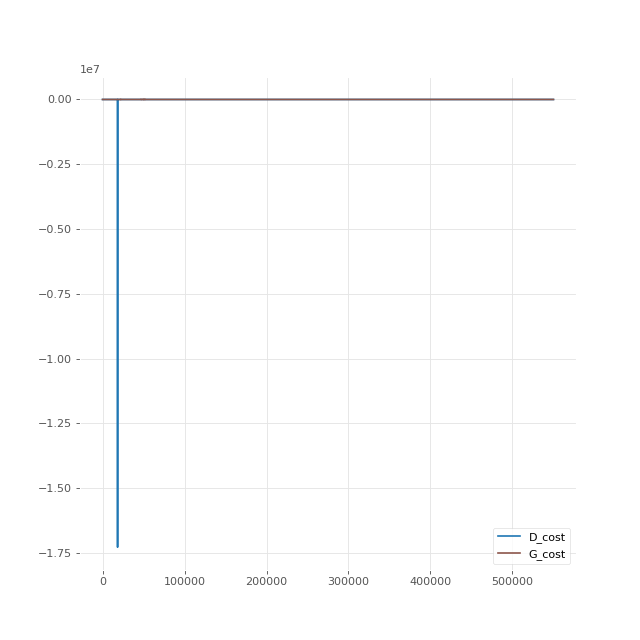
\includegraphics[width=\textwidth,center]{2019-04-30/mnist/info/plots/D_cost_G_cost.png}
   \caption{D_cost_G_cost.}
   \label{fig:.._.._notes_journal_figures_2019-04-30_mnist_info_plots-a}
\end{subfigure}
\begin{subfigure}[t]{0.48\textwidth}
   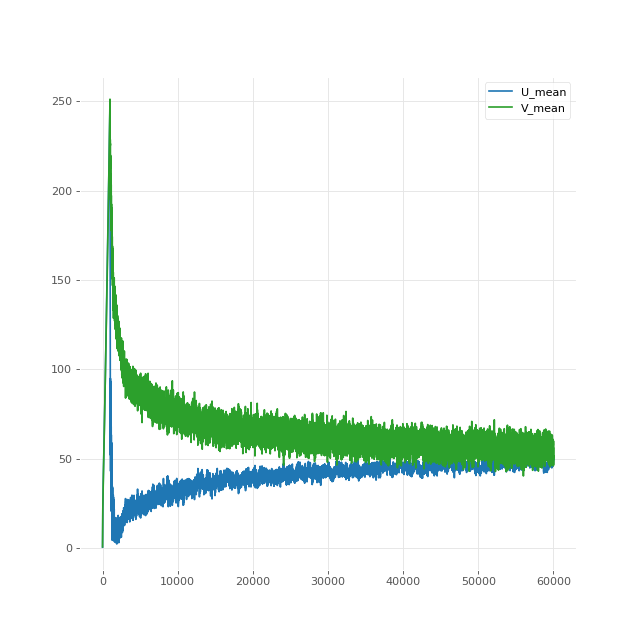
\includegraphics[width=\textwidth,center]{2019-04-30/mnist/info/plots/U_mean_V_mean.png}
   \caption{U_mean_V_mean.}
   \label{fig:.._.._notes_journal_figures_2019-04-30_mnist_info_plots-b}
\end{subfigure}
   \caption{.._.._notes_journal_figures_2019-04-30_mnist_info_plots}
   \label{fig:2019-04-30_mnist_info_plots}
\end{figure}
% \begin{figure}[!htbp]
   \centering
\begin{subfigure}[t]{0.48\textwidth}
   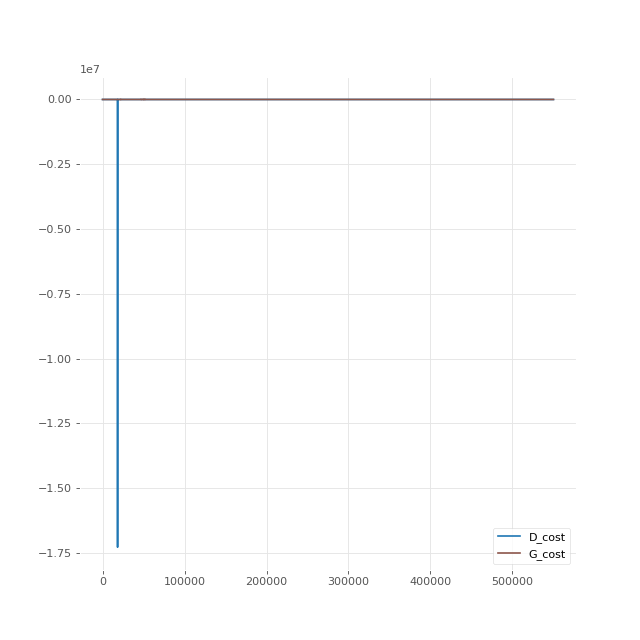
\includegraphics[width=\textwidth,center]{2019-04-30/mnist/info/plots/D_cost_G_cost.png}
   \caption{D_cost_G_cost.}
   \label{fig:.._.._notes_journal_figures_2019-04-30_mnist_info_plots-a}
\end{subfigure}
\begin{subfigure}[t]{0.48\textwidth}
   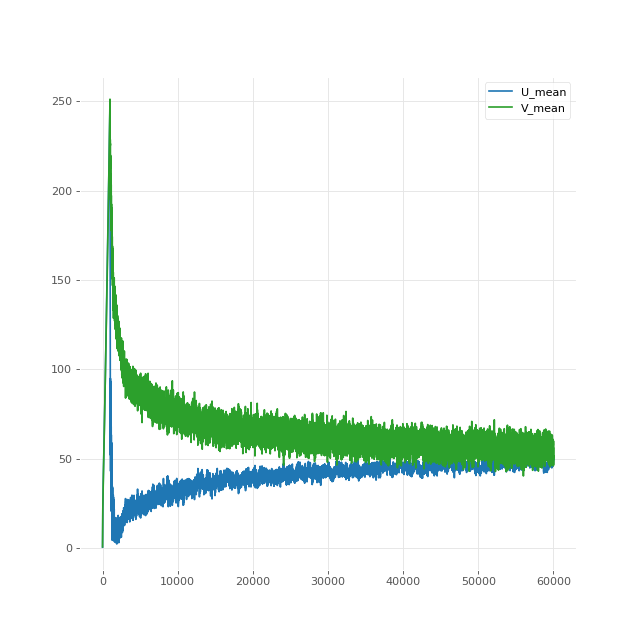
\includegraphics[width=\textwidth,center]{2019-04-30/mnist/info/plots/U_mean_V_mean.png}
   \caption{U_mean_V_mean.}
   \label{fig:.._.._notes_journal_figures_2019-04-30_mnist_info_plots-b}
\end{subfigure}
   \caption{.._.._notes_journal_figures_2019-04-30_mnist_info_plots}
   \label{fig:2019-04-30_mnist_info_plots}
\end{figure}
% \begin{figure}[!htbp]
   \centering
\begin{subfigure}[t]{0.48\textwidth}
   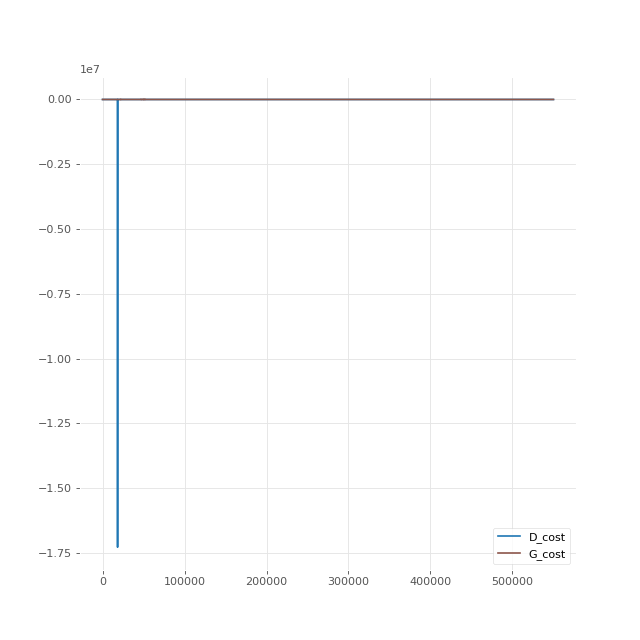
\includegraphics[width=\textwidth,center]{2019-04-30/mnist/info/plots/D_cost_G_cost.png}
   \caption{D_cost_G_cost.}
   \label{fig:.._.._notes_journal_figures_2019-04-30_mnist_info_plots-a}
\end{subfigure}
\begin{subfigure}[t]{0.48\textwidth}
   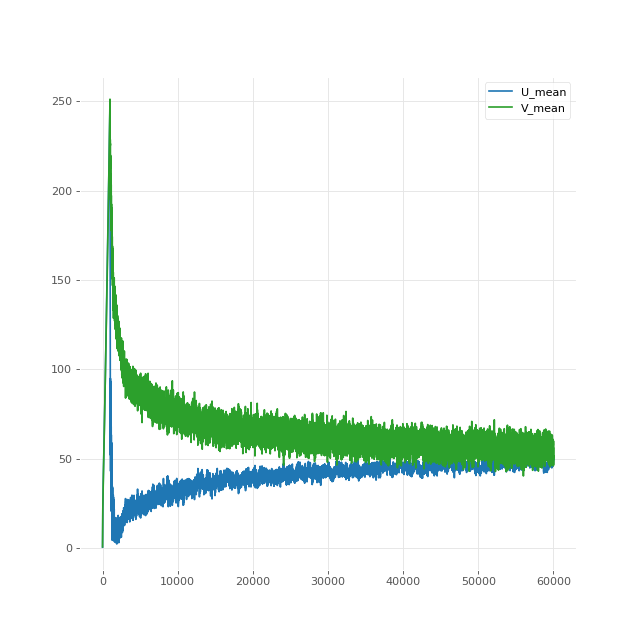
\includegraphics[width=\textwidth,center]{2019-04-30/mnist/info/plots/U_mean_V_mean.png}
   \caption{U_mean_V_mean.}
   \label{fig:.._.._notes_journal_figures_2019-04-30_mnist_info_plots-b}
\end{subfigure}
   \caption{.._.._notes_journal_figures_2019-04-30_mnist_info_plots}
   \label{fig:2019-04-30_mnist_info_plots}
\end{figure}
% \begin{figure}[!htbp]
   \centering
\begin{subfigure}[t]{0.48\textwidth}
   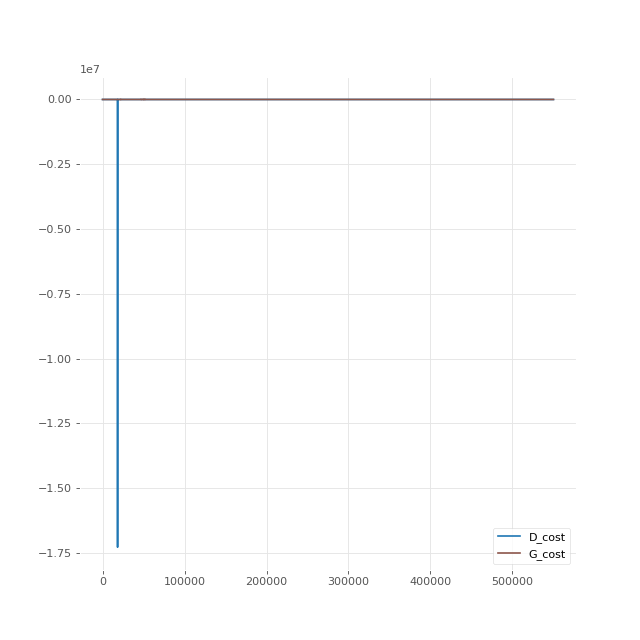
\includegraphics[width=\textwidth,center]{2019-04-30/mnist/info/plots/D_cost_G_cost.png}
   \caption{D_cost_G_cost.}
   \label{fig:.._.._notes_journal_figures_2019-04-30_mnist_info_plots-a}
\end{subfigure}
\begin{subfigure}[t]{0.48\textwidth}
   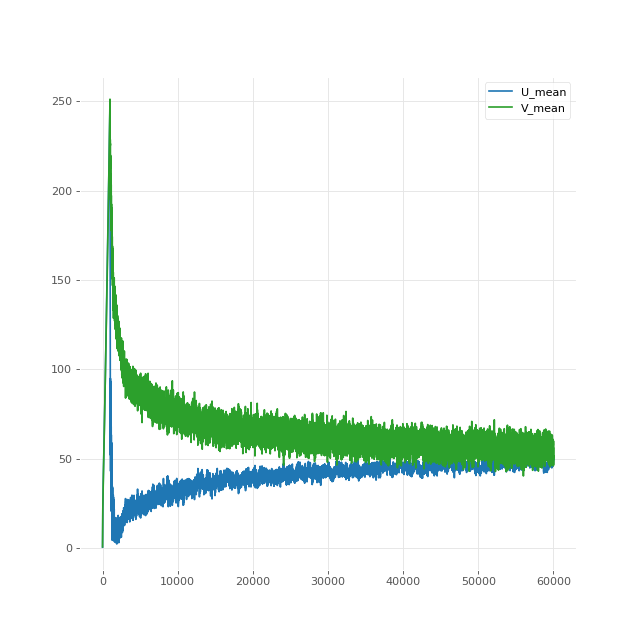
\includegraphics[width=\textwidth,center]{2019-04-30/mnist/info/plots/U_mean_V_mean.png}
   \caption{U_mean_V_mean.}
   \label{fig:.._.._notes_journal_figures_2019-04-30_mnist_info_plots-b}
\end{subfigure}
   \caption{.._.._notes_journal_figures_2019-04-30_mnist_info_plots}
   \label{fig:2019-04-30_mnist_info_plots}
\end{figure}
% \begin{figure}[!htbp]
   \centering
\begin{subfigure}[t]{0.48\textwidth}
   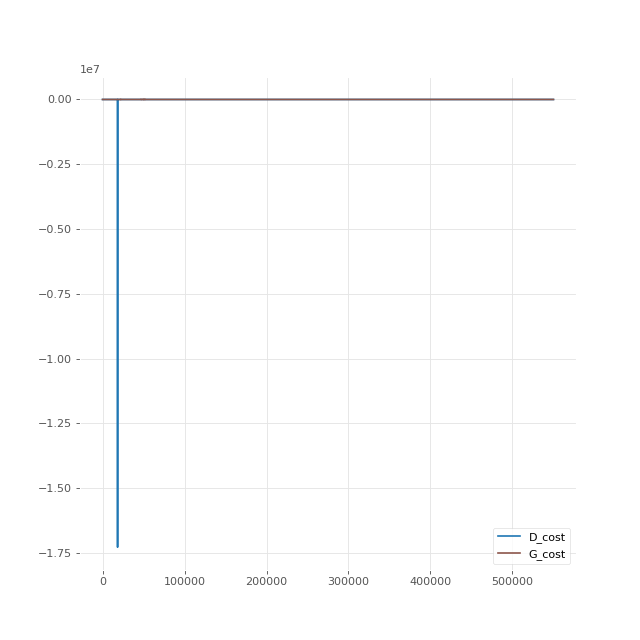
\includegraphics[width=\textwidth,center]{2019-04-30/mnist/info/plots/D_cost_G_cost.png}
   \caption{D_cost_G_cost.}
   \label{fig:.._.._notes_journal_figures_2019-04-30_mnist_info_plots-a}
\end{subfigure}
\begin{subfigure}[t]{0.48\textwidth}
   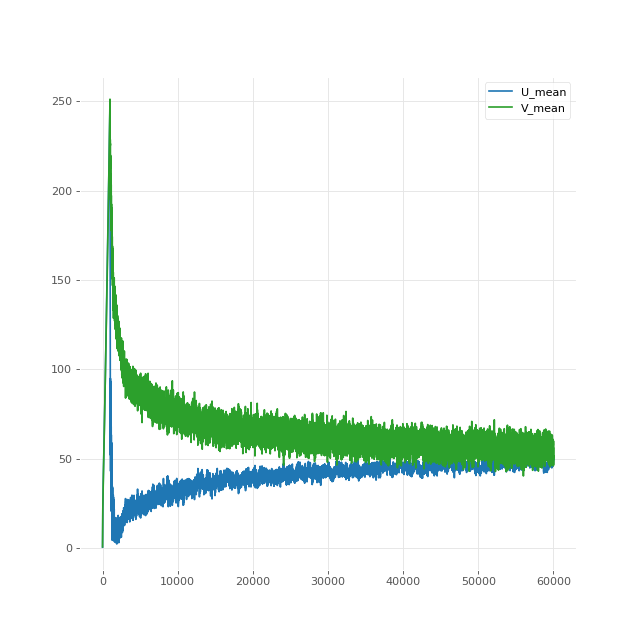
\includegraphics[width=\textwidth,center]{2019-04-30/mnist/info/plots/U_mean_V_mean.png}
   \caption{U_mean_V_mean.}
   \label{fig:.._.._notes_journal_figures_2019-04-30_mnist_info_plots-b}
\end{subfigure}
   \caption{.._.._notes_journal_figures_2019-04-30_mnist_info_plots}
   \label{fig:2019-04-30_mnist_info_plots}
\end{figure}
% \begin{figure}[!htbp]
   \centering
\begin{subfigure}[t]{0.48\textwidth}
   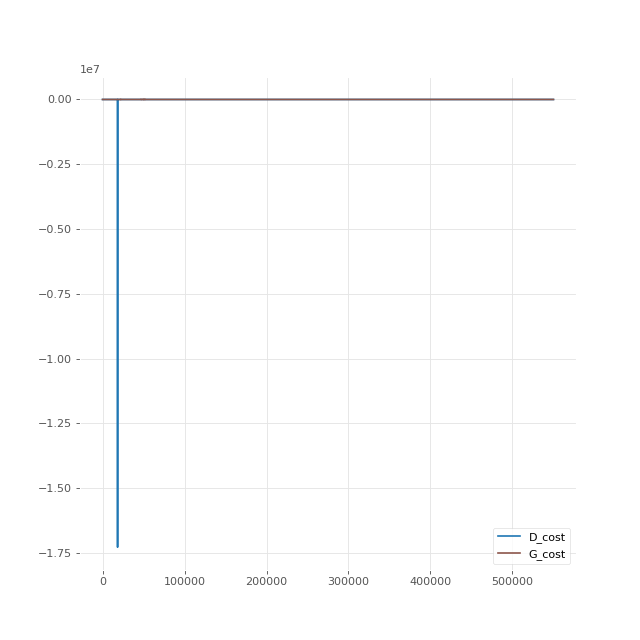
\includegraphics[width=\textwidth,center]{2019-04-30/mnist/info/plots/D_cost_G_cost.png}
   \caption{D_cost_G_cost.}
   \label{fig:.._.._notes_journal_figures_2019-04-30_mnist_info_plots-a}
\end{subfigure}
\begin{subfigure}[t]{0.48\textwidth}
   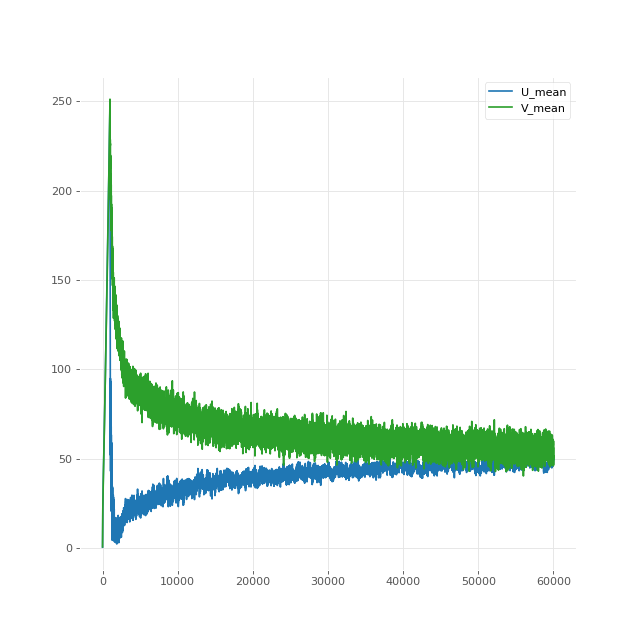
\includegraphics[width=\textwidth,center]{2019-04-30/mnist/info/plots/U_mean_V_mean.png}
   \caption{U_mean_V_mean.}
   \label{fig:.._.._notes_journal_figures_2019-04-30_mnist_info_plots-b}
\end{subfigure}
   \caption{.._.._notes_journal_figures_2019-04-30_mnist_info_plots}
   \label{fig:2019-04-30_mnist_info_plots}
\end{figure}
% \begin{figure}[!htbp]
   \centering
\begin{subfigure}[t]{0.48\textwidth}
   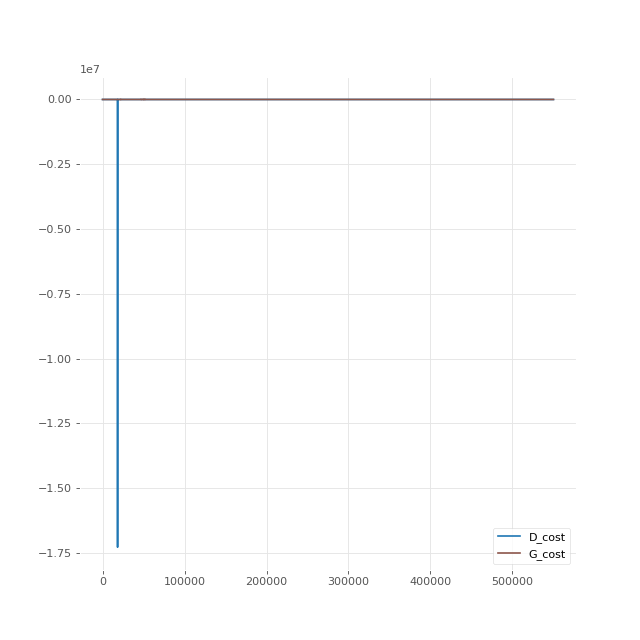
\includegraphics[width=\textwidth,center]{2019-04-30/mnist/info/plots/D_cost_G_cost.png}
   \caption{D_cost_G_cost.}
   \label{fig:.._.._notes_journal_figures_2019-04-30_mnist_info_plots-a}
\end{subfigure}
\begin{subfigure}[t]{0.48\textwidth}
   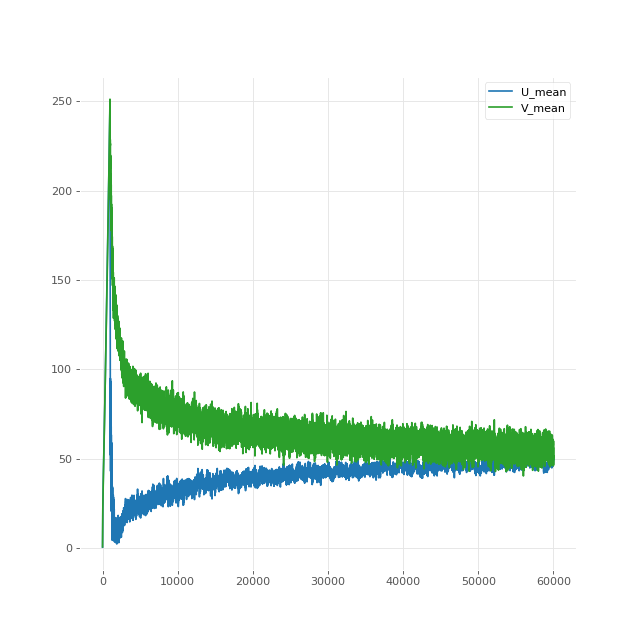
\includegraphics[width=\textwidth,center]{2019-04-30/mnist/info/plots/U_mean_V_mean.png}
   \caption{U_mean_V_mean.}
   \label{fig:.._.._notes_journal_figures_2019-04-30_mnist_info_plots-b}
\end{subfigure}
   \caption{.._.._notes_journal_figures_2019-04-30_mnist_info_plots}
   \label{fig:2019-04-30_mnist_info_plots}
\end{figure}
% \begin{figure}[!htbp]
   \centering
\begin{subfigure}[t]{0.48\textwidth}
   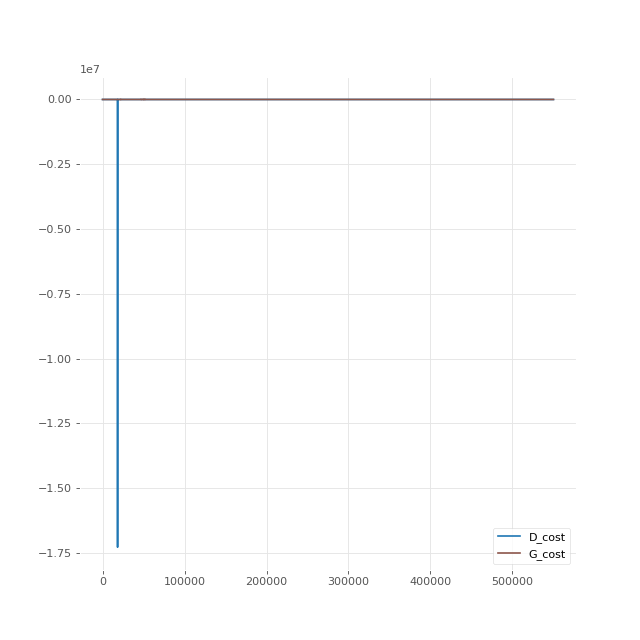
\includegraphics[width=\textwidth,center]{2019-04-30/mnist/info/plots/D_cost_G_cost.png}
   \caption{D_cost_G_cost.}
   \label{fig:.._.._notes_journal_figures_2019-04-30_mnist_info_plots-a}
\end{subfigure}
\begin{subfigure}[t]{0.48\textwidth}
   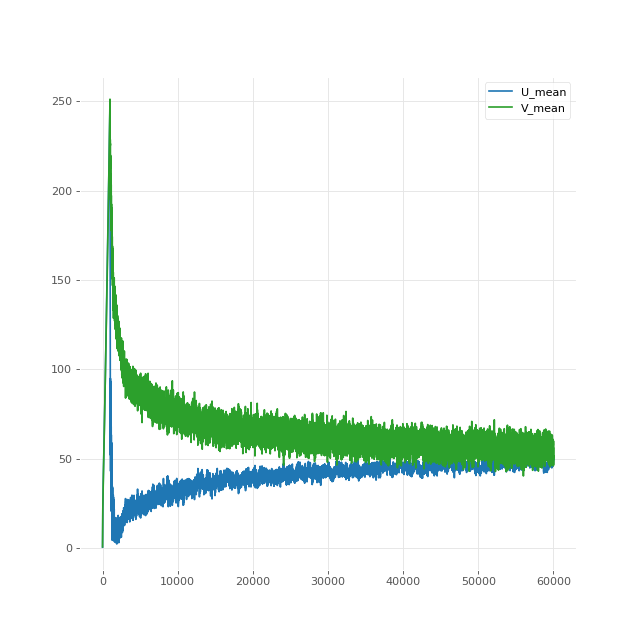
\includegraphics[width=\textwidth,center]{2019-04-30/mnist/info/plots/U_mean_V_mean.png}
   \caption{U_mean_V_mean.}
   \label{fig:.._.._notes_journal_figures_2019-04-30_mnist_info_plots-b}
\end{subfigure}
   \caption{.._.._notes_journal_figures_2019-04-30_mnist_info_plots}
   \label{fig:2019-04-30_mnist_info_plots}
\end{figure}
% \begin{figure}[!htbp]
   \centering
\begin{subfigure}[t]{0.48\textwidth}
   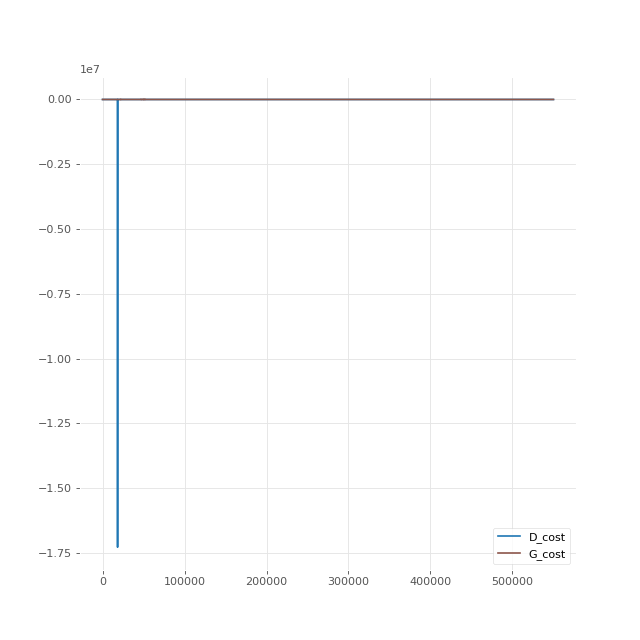
\includegraphics[width=\textwidth,center]{2019-04-30/mnist/info/plots/D_cost_G_cost.png}
   \caption{D_cost_G_cost.}
   \label{fig:.._.._notes_journal_figures_2019-04-30_mnist_info_plots-a}
\end{subfigure}
\begin{subfigure}[t]{0.48\textwidth}
   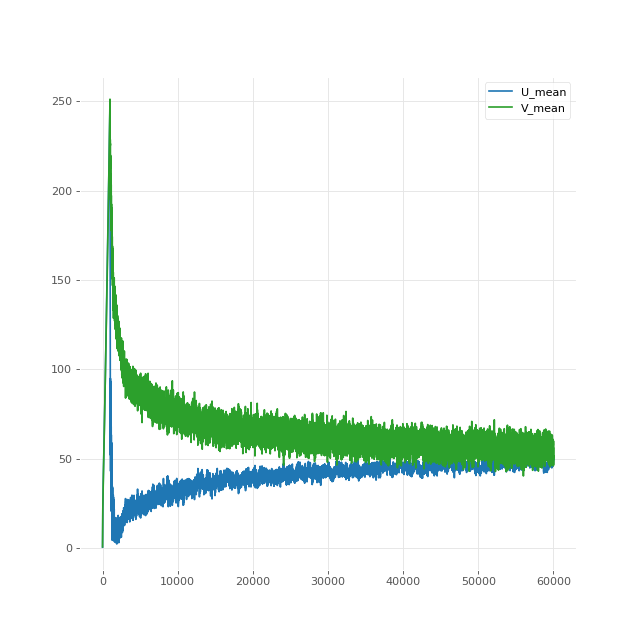
\includegraphics[width=\textwidth,center]{2019-04-30/mnist/info/plots/U_mean_V_mean.png}
   \caption{U_mean_V_mean.}
   \label{fig:.._.._notes_journal_figures_2019-04-30_mnist_info_plots-b}
\end{subfigure}
   \caption{.._.._notes_journal_figures_2019-04-30_mnist_info_plots}
   \label{fig:2019-04-30_mnist_info_plots}
\end{figure}

\section{After the meeting}
\begin{itemize}
    \item
        Try the expression of the dual network $Q_2$ similar to $Q_1$, on Gaussian and MNIST
    \item
        Crop the Celeba dataset like InfoGAN. Use extraction network to learn first unregularized and then regularized
    \item
        3DChairs ? optional first
    \item
        Mean / median images on MNIST
    \item
        Cretive ideas for the quantification metric of the informative models...
\end{itemize}

\printbibliography{}
\end{document}
